% !TEX root = ./main.tex
\begin{figure}[h]
    \centering
    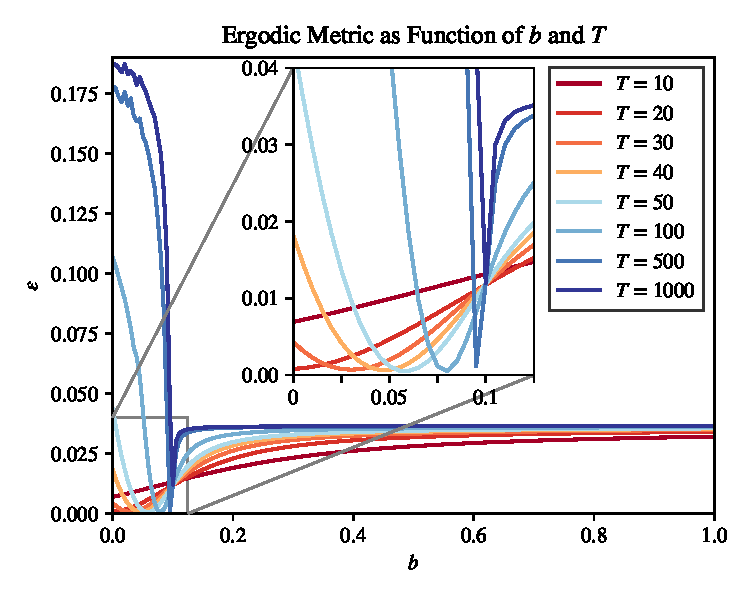
\includegraphics[]{ergodic_metric_final_colored.pdf}
    \vspace{-5mm}
    \caption{Plot of the ergodic metric $\varepsilon$ as a function of $b$ for different time horizons $T$, 
    for a choice of $k=10$ coefficients in each dimension and integrating for the spatial distribution coefficients over the domain $[-10,10]\times[-10,10]$.}
    \label{fig:ergodic}
\end{figure}
% Is there a most ergodic choice of b? 
% What is the most ergodic choice if you can choose both b and the time horizon T?
We can see that the most ergodic choice for $b$ is attained for a value between $0$ and $0.1$ regardless of the time horizon $T$. 
For the given $T=100$ seconds, the optmizer is attained at $b=0.08$.

If we can also choose $T$, then the most ergodic choice seems to be attained for $T\approx40$ seconds and $b\approx0.05$.